\documentclass[a4paper,12pt]{article} % Prepara un documento per carta A4, con un font di dimensione 12pt

\usepackage[italian]{babel} % Adatta LaTeX alle convenzioni tipografiche italiane,
% e ridefinisce alcuni titoli in italiano, come "Capitolo" al posto di "Chapter",
% se il vostro documento è in italiano
\usepackage[T1]{fontenc} % Riga da togliere se si compila con PDFLaTeX
\usepackage[utf8]{inputenc} % Consente l'uso caratteri accentati italiani

\usepackage{amssymb}

\usepackage{graphicx}

\frenchspacing % forza LaTeX ad una spaziatura uniforme, invece di lasciare più spazio
% alla fine dei punti fermi come da convenzione inglese

\title{Deduzione delle caratteristiche dell'alimentatore per giradischi THORENS TD 105} % \LaTeX è una macro che compone il logo "LaTeX"
% I commenti (introdotti da %) vengono ignorati

\author{A.G., in Imola.}
\date{26 Febbraio 2017}
% in alternativa a \date il comando \today introduce la data di sistema.



\begin{document}
\maketitle % Produce il titolo a partire dai comandi \title, \author e \date

\begin{abstract} % Questo è l'inizio dell'ambiente "abstract".
% L'ambiente abstract è fatto per contenere un riassunto del contenuto.
Partendo dal libretto di servizio (\emph{service manual}) del giradischi THORENS TD 105 si
deducono le caratteristiche che deve avere l'alimentatore per verificare
se possa essere impiegato un alimentatore diverso da quello di serie.
\end{abstract} % Qui termina l'ambiente ''abstract''



\section{Introduzione} %
L'alimentatore di serie del giradischi THORENS TD 105 è
un alimentatore AC/AC che ha uscita nominale di 10VAC;
la domanda a cui risponde questa relazione è: 
\begin{quote}
è possibile impiegare un alimentatore con uscita 12VAC
senza danneggiare il giradischi?
\end{quote}

\section{Analisi}
\begin{figure}[h]
\centering
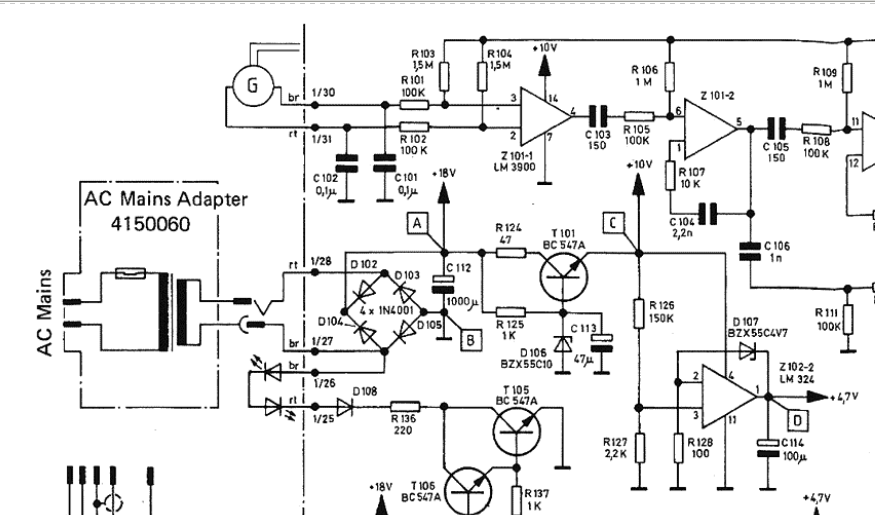
\includegraphics[width=\textwidth]{schematic_thorens}
\caption{Stralcio dello schema elettrico presente alle pagine 11 e 12 del libretto di servizio.}
\label{fig:schema}
\end{figure}

Il libretto di servizio \cite{libretto} riporta lo schema elettrico del giradischi ed
alcune informazioni per il controllo del corretto
funzionamento. Ci si riferisce allo schema elettrico di Figura \ref{fig:schema}. A pagina 15 del libretto si trovano queste indicazioni:

\begin{quote}
All voltages specified below are referred to 0 V (test point B)

Test point A -- STOP app. +20 VDC, 0.2 VAC
\end{quote}

quindi a giradischi acceso e piatto fermo connettendo il terminale \texttt{+}
del multimetro al test point \texttt{A}, il terminale \texttt{--} al test point \texttt{B}
e selezionando tensione in corrente continua, la lettura
deve essere circa +20 V. Da questa indicazione si ragiona a ritroso (\emph{reverse engineering})
con l'intento di stimare il valore di tensione tra i morsetti indicati
con \texttt{1/28} ed \texttt{1/27} che corrispondono all'avvolgimento secondario
del trasformatore che fa parte del \emph{AC Mains Adapter 4150060}.
Ignorando il ripple presente al test point \texttt{A}, alla tensione 
misurata sul test point \texttt{A} va aggiunta la caduta di tensione
che si ha sulla coppia di diodi tipo 1N4001 nel loro stato di 
conduzione e che costituiscono metà del ponte raddrizzatore, 
tipicamente si può considerare una caduta in conduzione di
circa 0.8V\cite{datasheet}, questo porta ad una tensione tra \texttt{1/28} e \texttt{1/27}
di 21.6V; questo valore è quindi il valore di picco
dell'onda AC, il valore efficace è $\sqrt{2}=1.414$
volte più basso e quindi è $\frac{21.6}{1.414}=15.3$V.\\

Quindi, siccome tipicamente le indicazioni per la AC
sono espresse come valore efficace (vedi per esempio \cite{norma}) si conclude che
un alimentatore AC/AC con uscita 12VAC non dovrebbe danneggiare
il giradischi perché  produrrebbe al test point \texttt{A} una tensione
inferiore a quella dichiarata nel libretto di servizio a fronte del
normale funzionamento dello stesso.\\

\begin{figure}[h]
\centering
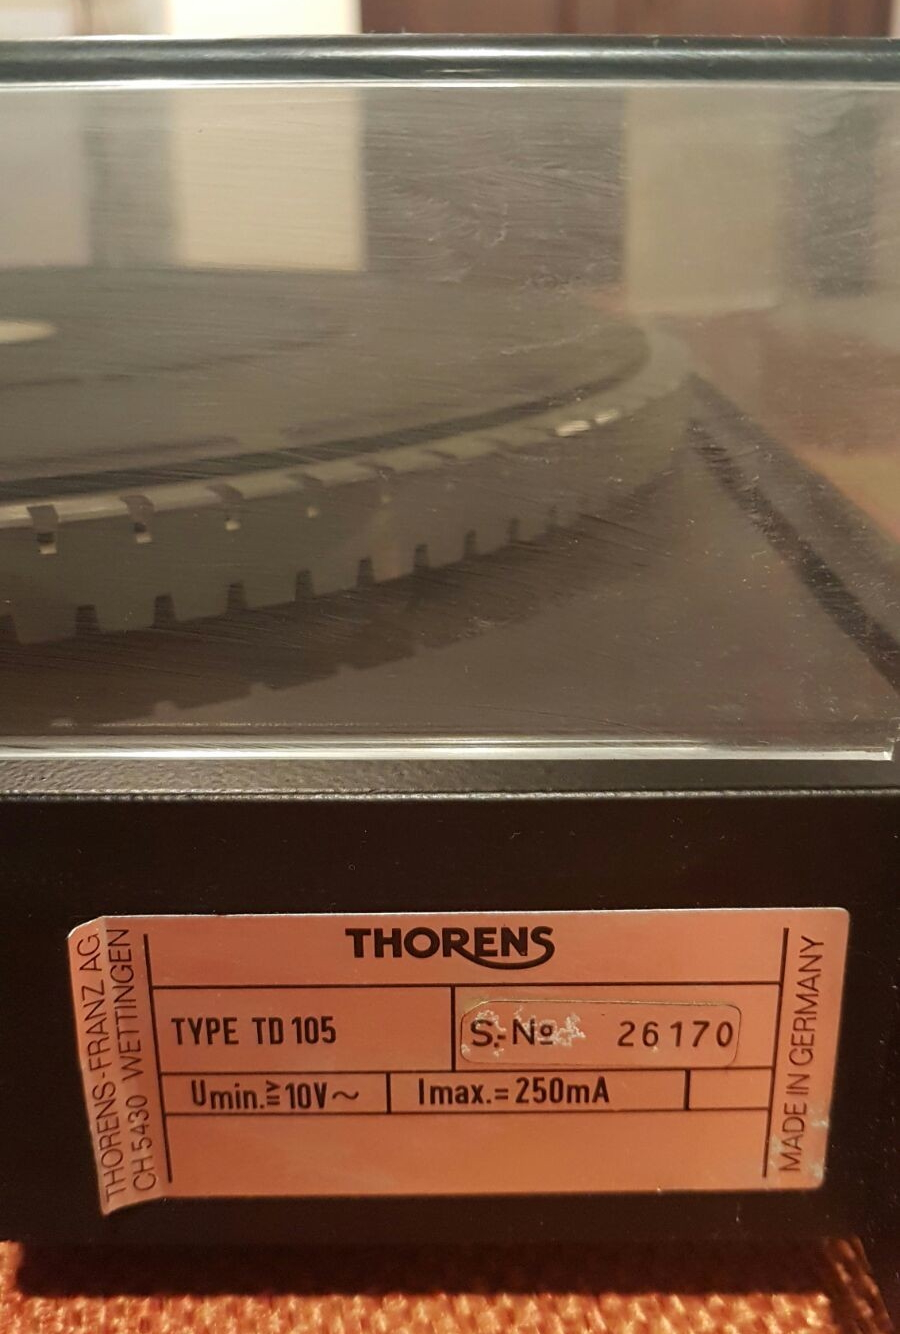
\includegraphics[width=7cm]{thorens_label}
\caption{Etichetta sul retro del giradischi.}
\label{fig:label}
\end{figure}

Inoltre l'etichetta visibile in Figura \ref{fig:label} riporta la dicitura
$U_{min}\geqq10V\sim$ dove il simbolo 
$\geqq$ significa ``maggiore o uguale'': quindi anche
questo suppporta l'ipotesi che sia possibile impiegare una
tensione maggiore di 10VAC per alimentare il giradischi.

\begin{thebibliography}{9}
\bibitem{libretto} 
THORENS Service Manual
\\TD 104 / TD 105 Turntables

\bibitem{datasheet}
1N4001, 1N4002, 1N4003,
1N4004, 1N4005, 1N4006,
1N4007
\\Axial Lead Standard Recovery Rectifiers.
\\ ON Semiconductor
\\\texttt{http://www.onsemi.com/pub\_link/Collateral/1N4001-D.PDF}

\bibitem{norma}
NORMA TECNICA
\\CEI 8-6:1998-04



\end{thebibliography}

\end{document}
